\documentclass[9pt,journal,compsoc]{IEEEtran}
\usepackage[english]{babel}
\usepackage[utf8]{inputenc}
\usepackage{cite}
\usepackage{amsthm}
\usepackage{amsmath}
\usepackage{amssymb}
\usepackage{graphicx}
\usepackage{array}
\usepackage{algorithmic}
\usepackage{url}

% correct bad hyphenation here
\hyphenation{op-tical net-works semi-conduc-tor}

\newtheorem{mydef}{Definition}

\begin{document}

\title{\huge Categorisation of Urban Water Consumptions}

% Author information
\author{
	\IEEEauthorblockN{Joaquim Leitão\IEEEauthorrefmark{1}}
	
	\IEEEauthorblockA{\IEEEauthorrefmark{1}jpleitao@dei.uc.pt \\ CISUC, Department of Informatics Engineering, Univesity of Coimbra, Portugal}
}

% The paper headers
\markboth{Connectivity and Pattern Recognition, 2016-2017}{Connectivity and Pattern Recognition, 2016-2017}


\IEEEtitleabstractindextext{
\begin{abstract}
	Lol, here goes the abstract
\end{abstract}

\begin{IEEEkeywords}
	Water Consumption Patterns, Clustering, Time series, Pattern Recognition.
\end{IEEEkeywords}
}


% make the title area
\maketitle
\IEEEdisplaynontitleabstractindextext
\IEEEpeerreviewmaketitle


\IEEEraisesectionheading{\section{Introduction}\label{sec:introduction}}

\IEEEPARstart{I}{n} most cities and urban areas investment in equipment related to water supply and drainage is substantial, being responsible for a considerable share of the budget of many municipalities.

Substantial attention has been given to the construction and installation of new pipe and sewage infrastructures, as well as to maintenance operations on existing infrastructures; however, relatively small efforts have been made to study water consumption patterns in these environments.

Indeed, understanding and accurately predicting such behaviours is extremely important to water companies, as it allows them to improve the management of their infrastructures, namely water storage facilities (such as water tanks and towers): Many water utilities repeatedly overestimate the volume of water needed to supply the population of a given region. Therefore, water companies tend to operate existing water storage tanks close to their full capacity, resulting in higher energy-related costs (since water has to be pumped into the tanks) and in larger volumes of retained water. 

By being capable of characterising water consumption patterns in a given region water companies could adjust water volumes in existing storage tanks\footnote{For obvious reasons this volume must always be overestimated; however, such overestimation could be better controlled.}, improving the management of their finances and reducing excess water volumes retained in storage tanks.

The current work aims at categorising water consumptions in a given region of a median size city, contributing towards an improved understanding and knowledge of water consumption patterns. Therefore, in this work, historic water consumptions are intended to be processed and organised in different groups according to their similarity.

In the field of pattern recognition, tasks of this nature are referred to as \emph{clustering} approaches. Since a time-ordered series of data (water consumptions, in this case) is intended to be processed and clustered, the proposed problem can be considered as \emph{time series clustering}. In this sense, it is important to define this term. We present a definition proposed by Aghabozorgi \emph{et al.} \cite{aghabozorgi2015time}:

\begin{mydef}[Time Series Clustering]
	"Given a dataset of n time series data $D = \{F_{1}, \cdots , F_{n}\}$, time series clustering can be defined as the process of unsupervised partitioning of $D$ into $C = {C_{1}, \cdots , C_{k}}$ in such a way that homogeneous time series are grouped together based on a certain similarity measure."
\end{mydef}

The remainder of this document is organised as follows: Section \ref{objectives} presents the main objectives of this work. In section \ref{dataset_description} water consumption data used in this work is briefly presented. The methodology adopted throughout this work is discussed in section \ref{methodology}. Sections \ref{} to \ref{} cover the main steps of the work, presented in the methodology section. Finally, section \ref{conclusions} concludes this document.

\textbf{FIXME: Review outline}

\section{Objectives}
\label{objectives}

The main objective of the proposed work is related with the categorisation of urban domestic water consumptions in a given region of a median size city.

That is, taking into account information about an entire civil year (from January 1st to December 31st) the system must be capable of identifying recurrent consumption patterns and determine the moments in time when such patterns were repeated: an intuitive (and somewhat expected) result is that water consumptions during summer months will have a similar shape, which substantially differs from those recorded during winter months. This could be justified by the fact that many people in that region usually spend summer months away, on vacation.

In this sense, the appropriate steps of a pattern recognition system will be considered, namely: (i) data pre-processing; (ii) pattern recognition techniques - in this case clustering techniques; (iii) analysis of the experimental results.

\section{Dataset Description}
\label{dataset_description}

The dataset to be used in the proposed project contains domestic water consumptions in different regions of a median size city. The available data corresponds to the entire 2016 year and was obtained as a result of a collaboration with \emph{Águas de Coimbra}\footnote{\url{http://www.aguasdecoimbra.pt/}}, the public water company in the city of Coimbra, Portgual.

Water consumption's measurement is carried out in strategic locations of the city, through measurement and control zones - \emph{ZMC}\footnote{Or in portuguese, \emph{Zonas de Medição e Controlo}.}. These infrastructures provide a more efficient management of the water distribution systems, enabling the network's management in logical zones of analysis and allowing the adoption of measures to control water losses.

Collected data corresponds to a time series of total water volume distributed to the region in question - recorded as a floating point number whose units are $m^{3}/h$. Therefore, pairs of values $(time, volume)$ are provided. The collection time is provided in the format \emph{dd/mm/yyyy HH:MM:SS}.

During the data acquisition equipment errors and malfunctions can occur, resulting in the failure to record the total consumptions. In such moments, a value of \emph{"n/a"} is presented for the total distributed water volume, signalling the missing value. The developed pattern recognition system must adopt proper techniques to deal with these missing values.

\section{Methodology}
\label{methodology}

To accomplish the mentioned objectives the following steps were considered in the developed work:

\begin{enumerate}
	\item \textbf{Time Series pre-processing}, comprising two major tasks: computing the unit of analysis for the time series; and imputing missing values
	
	\item \textbf{Time Series Representation}, consisting in the application of dimensionality reduction techniques. As will be explained later in this section, both raw time series data and dimensionality reduced time series data is intended to be clustered, in order to compare the results obtained with both methods.
	
	\item \textbf{Segmentation of water consumptions}, consisting in the application of clustering techniques to group similar samples together.
	
	\item \textbf{Results analysis and assessment}
\end{enumerate}

Extensive research has been made in the field of time series clustering, resulting in the adoption and proposal of a wide variety of clustering approaches and techniques. In a 2015 survey on time series clustering, Aghabozorgi \emph{et al.} \cite{aghabozorgi2015time} highlights techniques such as \emph{hierarchical clustering}, \emph{k-means clustering} and \emph{k-medoids clustering}. Other techniques have also been applied, such as neural networks and variations of the mentioned algorithms, namely of \emph{k-means} ans \emph{k-medoids}.

Determining the most appropriate technique to be applied in our problem is far from being an easy task. The same methods applied on data of different natures can produce completely different results, and the same can even be considered with data of the same nature, but collected from distinct sources and (most probably) with a different methodology.

As a result, in the current work, different techniques are intended to be explored in an attempt to determine the ones that appear to be more suitable to the collected data. These techniques fall in four distinct categories: \emph{Missing Data Imputation}, \emph{Time Series Representation}, \emph{Time Series Distance Metrics} and \emph{Clustering Algorithms}.
 
Regarding missing data imputation, three distinct techniques are considered to be applied to provide sounding estimations for missing water consumptions data: fitting a polynomial expression, fitting an ARIMA model or the application of Kalman Filters.
	
Distance computation between raw time series data tends to be an heavy task in terms of computational resources. The main reason for this has to do with the high dimensionality of time series data. In this sense, in some publications the application of dimensionality reduction techniques has been explored. In the scope of this work both raw time series data and reduced dimensionality time series data is intended to be applied. Regarding dimensionality reduction techniques, \emph{Principal Components Analysis} and \emph{Stacked Autoencoders} are intended to be explored.
	
When dealing with raw time series, the use of more traditional distance metrics, such as the euclidean distance, has been shown to fail in capturing similarities in the series' shape. Alternative distance metrics, among which \emph{Dynamic Time Warping} (DTW) \cite{chu2002iterative} is highlighted, have been extensively adopted when dealing with raw time series data \cite{petitjean2014dynamic, izakian2015fuzzy} and is considered a more robust distance metric for time series \cite{wang2013experimental}. Nevertheless, euclidean distance is still applied in time series clustering works, specially if dimensionality reduction techniques are employed. An example of such application can be found in the work of Abreu \emph{et al.} \cite{abreu2012using}. In this sense, DTW is intended to be used when dealing with raw time series data, whereas the euclidean distance will be the choice for the dimensionality reduced data.
	
Clustering Algorithm: \textbf{FIXME: Para já estou apenas a considerar HC + K-Means e apenas vario a metrica de distancia e a forma como calculo os centroides. No entanto posso vir a considerar um outro algoritmo, o TADPole, que aparentemente existe em R e é batante utilizado - Para já deixar este ponto em standby}

\textbf{FIXME: Adicionar uma tabela com os grupos de testes que fizémos}

\textbf{FIXME: Acho que é melhor colocar esta tabela na sua propria secção depois da secção de clustering! Alterar referências a esta tabela! Dizer também que apenas fizémos um conjunto de testes para reduced dimensionality por questões de tempo, mas que seria interessante aplicar outras métricas no calculo dos centroides, nomeadamente aplicar o medoid!}

\section{Time Series Pre-Processing}
\label{pre_processing}

As stated in section \ref{methodology}, time series pre-processing comprises two main iterations: computing the unit of analysis of the time series and imputing missing values in time series' readings. These steps will be covered in more detail in their own subsections.

\subsection{Unit of Analysis}

When identifying patterns of recurrent behaviour in time series data it is important to determine the periods of time with the higher contributions to the overall signal. In other words, the most intense and important periods of time are sought.

Similarly to the works of Abreu \emph{et al.}\cite{abreu2012using} and Calabrese \emph{et al.}\cite{calabrese2010eigenplaces}, a \emph{Fourier} analysis can be conducted on the collected time series data to determine the frequencies with higher contribution. In this sense, a \emph{Fast Fourier  Transform} (FFT) was performed on the time series data. 

Analysing the results of such transformation, it was determined that the frequency with the largest contribution to the resulting signal was the frequency 0 $Hz$. Even though this may seem an unexpected result, a valid explanation can be found: by performing the FFT of a given signal, the frequency with higher contribution is usually an approximation of the fundamental frequency. As the signal being analysed (the time series data) is not periodic, its fundamental period is infinite, rendering its fundamental frequency to be 0 $Hz$. In such scenarios, the second frequency with higher contribution is usually considered as the unit of analysis. In this case such a frequency was around $24h$, suggesting this to be the unit of analysis.

With this finding, an aggregation of the time series values was conducted: the values of the original time series were recorded with a one-minute interval; since the unit of analysis is $24h$, each sample to be clustered contains readings of one day, with an interval of $1h$\footnote{Therefore, each sample consists in a list of 24 values, one per hour. These individual hourly consumptions were obtained simply by adding all partial consumptions in the same hour.}.

\subsection{Missing Data Imputation}

In almost all real-life applications, errors in the data collection procedures are prompted to occur, forcing data analysis and processing methods to properly deal with missing and invalid values. Substantial research has been performed on the topic of missing data imputation, resulting in different methods and techniques being proposed and tested in a variety of problems.

Nevertheless, choosing a valid missing data imputation technique to be applied in a given problem is far from being an easy task. The same method can have completely distinct performances when applied to different data, of diverse natures and/or collected in different ways. In the particular case of this work, no previous studies of the performance of missing data imputation methods had been conducted on the collected data. As a result, a choice was made to browse the literature on this topic and test the application of the most cited and used ones in the collected data.

Steffen \emph{et al.}\cite{moritz2015comparison} studied the application of different missing data imputation methods on univariate time series. In their work, the authors obtained interesting results for approaches exploring linear interpolation, ARIMA and SARIMA models and Kalman Filters. 

Alternative methods can also be considered. Usually more active in time series prediction and classification, techniques featuring artificial neural networks, decision tress or k-nearest neighbours\cite{troyanskaya2001missing, yu2014short} can also be applied to compute estimations for missing values. In addition, traditional time series analysis methods such as autocorrelation and trend analysis have also been applied\cite{abreu2012using}, as well as expectation-maximization and multivariate algorithms on lagged data\cite{moritz2015comparison}.

Inspired by the results reported on the literature, and after an initial study of the different methods, a choice was made to select the following three missing data imputation methods for further analysis: (i) linear interpolation; (ii) ARIMA; (iii) Kalman Filter.

At this point, the goal of this analysis was to studying the performance of these methods when applied to the collected data. This study was conducted as follows: Initially individual samples were divided into samples that contained missing values and samples without missing value\footnote{The reader must keep in mind that individual samples consist in a list with water consumptions for a given day, featuring hourly values.}. For each complete sample missing values were artificially introduced. Each method was then applied to the individual samples and the correctness of their imputations was assessed using the \emph{root mean squared error} (rmse) metric.

Overall the Kalman Filter produced better estimates than the competing alternatives: An average rmse of about $263.83$ was registered (against a rmse of about $571.37$ for the ARIMA model and $12403.17$ for the linear interpolation), and the Kalman filter produced better daily estimates (smaller rmse on individual samples) in 189 days (against 72 for the ARIMA model and only 4 for the linear interpolation).

Based on such results the Kalman Filter was chosen as the imputation approach for our data. Therefore, for each day where missing data were registered, a Kalman Filter model was computed and estimations for the missing data in that day were obtained.

\section{Time Series Representation}
\label{time_series_representation}

When working with high dimensional data, computational requirements grow both in terms of memory and execution time: if each time series contains more values then it will require more space in memory and, therefore, if a larger number of time series is intended to be clustered or processed in some way substantially more memory may be required to load all the time series data. In addition, specially in the case of clustering, distance computation between data samples is often performed; if a larger number of samples is considered, each comprising several dimensions, distance computation between pairs of samples will take longer to compute, as will the overall process.

Another motivation for seeking alternative time series representations, as pointed out by Aghabozorgi \emph{et al.}\cite{aghabozorgi2015time}, has to do with the fact that when measuring the distance between raw time series samples highly unintuitive results may be gathered resulting in the clustering of series similar in noise, instead of shape. It must be noticed that the adopted distance metric highly influences the clustering results.

In this sense, several time series representation methods have been proposed in the literature. Aghabozorgi \emph{et al.} presents a taxonomy comprising four main categories: i) Data adaptive; (ii) Non-data adaptive; (iii) Model-based; and (iv) Data dictated. The choice of time series representation has a big impact in the outcome of the clustering exercise, in both quality and execution time. Furthermore, time series representation also affects the choice of distance metric (also called dissimilarity function).

In the specific clustering problem being tackled in this work, where time series containing similar behaviours are intended to be grouped together, one of the major challenges to be face has to due with the dissimilarity function (that is, how to determine that two time series are close together). Even though it is computationally expensive, the \emph{Dynamic Time Warping} (DTW) distance metric is quite popular\cite{liao2005clustering, aghabozorgi2015time}.

As the DTW targets time sequences, it can be concluded that a substantial number of approaches adopt a raw time series representation. Dimensionality Reduction (DR) techniques such as \emph{Principal Components Analysis} (PCA) have also been explored \cite{abreu2012using} in an attempt to represent time series samples in fewer dimensions, thus reducing the computational burden of distance computation. As the application of DR techniques loses the temporal sequence of the data, alternative distance metrics need to be considered.

In light of the discussion carried out in this section, in the scope of the current work, it is intended to explore clustering performance obtained using two distinct time series representation approaches: (i) \textbf{Raw time series representation}, featuring the use of the popular \emph{Dynamic Time Warping} distance metric; (ii) \textbf{"Dimensionality-Reduced" time series representation}, featuring the use of the classical \emph{Euclidean} distance.

\subsection{Raw Time Series Representation}

With respect to the \emph{raw} time series representation not much needs to be added to what has already been mentioned. Initially, this representation can be seen as considering raw collected time series values.

Taking into account the pre-processing steps mentioned in section \ref{pre_processing}, imputed time series corresponding to daily lists of hourly water consumption readings should be considered at this point; however, an additional step must be considered: when working with raw time series data, performing a \emph{Z-Normalization} of the data can significantly improve distance computation results with the DTW metric\cite{mueen2016extracting}.

As a result, when working with raw time series representation, a \emph{Z-Normalization} of the data was conducted. The \emph{Z-Normalization} can be defined as:

$$X = \frac{X - MEAN(X)}{STD(X)} $$

\subsection{Dimensionality Reduction for Time Series}

Regarding the application of dimensionality reduction techniques to time series data, two popular algorithms of this nature were compared: \emph{PCA} and \emph{Stacked Autoencoders} (SAEs). The comparison was based on the rmse on reconstruction and on visual inspection of the reconstructed series.

In PCA the target number of features was selected as a function of the percentage of explained data variance. In this sense, principal components capable of representing $80\%$ of the data variance were selected, yielding a reduced dimensionality of 3 features.

SAEs were then trained for dimensionality reduction, targeting the same number of features as PCA. Different network architectures were considered while training the SAEs (that is, different number of autoencoders with different numbers of neurons per hidden layer, different activation functions, etc); however, in the best scenarios, SAEs were only capable of getting close to PCA in terms of reconstruction error, producing reconstructed time series considerably more distant to the original ones than PCA.

It is also worth mentioning at this point that both PCA and SAEs approaches were tested with normalised data, using the \emph{Min-Max} method. Figure \ref{day3_reconstruction} presents a reconstruction of water consumptions for one day using both a PCA decomposition and Stacked Autoencoders.

\begin{figure}[ht]
	\centering
	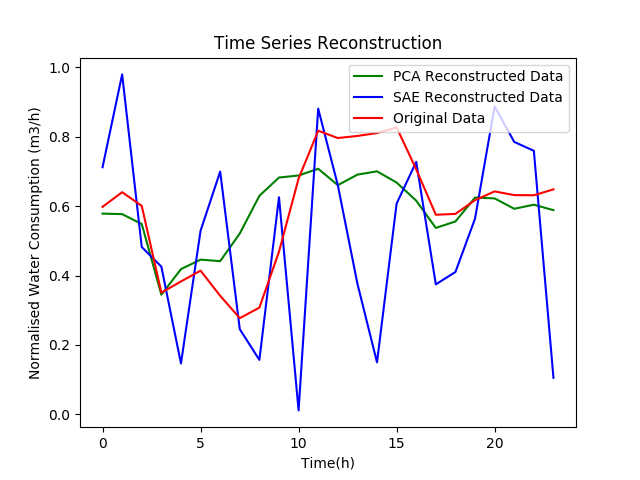
\includegraphics[scale=0.5]{images/pca_sae_day3.png}
	\caption{Reconstruction of water consumptions for one day using a PCA decomposition and a Stacked Autoencoder.}
	\label{day3_reconstruction}
\end{figure}

From the analysis of figure \ref{day3_reconstruction} it is clear that, even though SAEs may be able to reconstruct the original data with an error close to PCA, SAEs fail in capturing the shape and tendency of the series. As a proper learning could not be obtained with SAEs, PCA was the dimensionality reduction technique chosen to be applied in the experiments and exercises carried out in the remainder of this work.

\section{Clustering}

Dizer que escolhemos HC + K-Means \textbf{FIXME: TADPole?}

why and how!!!

Mostrar resultados HC

A major characteristic of K-Means clustering is that, depending on how the initial cluster centroids are computed, different results in each run of the algorithm (for the same value of the parameter K) may be produced. This is specially true if a random initialisation is performed.

As a result of this characteristic, K-Means clustering is usually executed several times for the same value of K and the initial cluster selection that produces better results is chosen. The question that immediately raises from such a statement is how to determine if one cluster selection is better than another? To answer this question, Anil Jain \cite{jain2009data} proposed the execution of the K-Means algorithm several times, for the same value of $k$, keeping the partition that produced the smallest squared error.

In K-Means, clusters are sought so that their within-cluster distances are minimised and between-cluster distances maximised. Indeed, this is exactly the same evaluation performed in the computation of the silhouette coefficient. In this sense, Jain's suggestion was slightly adjusted, to keep the partition with the higher silhouette coefficient value, instead of the lowest squared error.

Therefore, for each of the tests presented in table \ref{} \textbf{FIXME: Referência tabela a adicionar na secção 4} where the K-Means algorithm was used, 10 repetitions for the algorithm were considered for each value of $k$ defined. After the 10 repetitions, only the partition with the highest silouette coefficient value was kept.

\section{Summary of the Experiments}

Colocar a tabela


\section{Results Assessment}

\textbf{FIXME: Texto introdutório}

\subsection{Initial Results Analysis}

Dizer que os resultados obtidos para cada uma das combinações de métodos apresentados anteriormente (que podem ser consultados na tabela da secção 4) foram avaliados segundo X métricas: \textbf{FIXME: Apresentar métricas num itemize e fazer uma breve descrição, colocar fórmulas, dizer que valores são bons, etc}

Fazer uma reflexão sobre os resultados e dizer quais aqueles que merecem ser mais estudados.

\subsection{Further Results Analysis}

Apresentar novas métricas, resultados e reflexão

Meter gráficos aqui

\section{Conclusion}
\label{conclusions}


\bibliographystyle{ieeetr}
\bibliography{bibliography.bib}

\end{document}